\videotitle{Speedup Techniques}

%-------------------------------------------------


%----------------------------------------------------
\myframe{Overview of NAS Speedup Methods}{

	\myit{
		\item Multi-fidelity optimization
\bigskip
		\item Learning curve prediction
\bigskip
		\item Meta-learning across datasets
\bigskip
		\item Network morphisms \& weight inheritance
\bigskip
		\item Weight sharing \& the one-shot model
	}
}
%----------------------------------------------------

%----------------------------------------------------
\myframe{NAS Speedup Technique 1: Multi-fidelity optimization}{
    \myit{
    	\item \alert{Analogous to multi-fidelity optimization in HPO}
    	\myit{
    		\item[-] Many evaluations for cheaper fidelities (less epochs, smaller datasets, down-sampled images, shallower networks, etc)
    		\item[-] Fewer evaluations necessary for more expensive fidelities
    	}
\medskip
\pause
		\item \alert{Compatible with any blackbox optimization method}
    	\myit{
    		\item[-] Using random search: ASHA \lit{\href{https://arxiv.org/pdf/1902.07638.pdf}{Li and Talwalkar. 2019}}
    		\item[-] Using Bayesian optimization: BOHB \lit{\href{https://arxiv.org/pdf/1807.06906.pdf}{Zela et al. 2018}}
    		\item[-] Using differential evolution: DEHB \lit{Awad et al. under review}
    		\item[-] Using regularized evolution: progressive dynamic hurdles \lit{\href{https://arxiv.org/pdf/1901.11117.pdf}{So et al. 2019}}
		}
\medskip
\pause
    	\item \alert{Often used for joint optimization of architecture \& hyperparameters}
    	\myit{
    		\item[-] Auto-Pytorch \lit{\href{https://www.automl.org/wp-content/uploads/2019/05/AutoML_Book_Chapter7.pdf}{Mendoza et al. 2019}; \href{https://arxiv.org/pdf/2006.13799.pdf}{Zimmer et al. 2020}}
    		\item[-] ``Auto-RL'' \lit{\href{https://openreview.net/pdf?id=ByfyHh05tQ}{Runge et al. 2019}}
    	}
    	
%    	LC prediction, extrapolation, multi-multi-fidelity, etc
    }
}
%----------------------------------------------------

%----------------------------------------------------
\myframe{NAS Speedup Technique 2: Learning Curve Prediction}{
    \myit{
		\item \alert{Analogous to learning curve prediction in HPO}
    	\myit{
    		\item[-] Observe initial learning curve and predict performance at the end
    		\item[-] Can use features of the architecture as input (just like hyperparameters as inputs)  
    	}
\pause
\medskip
    	\item \alert{Often used for joint optimization of architecture \& hyperparameters}
\medskip
		\item \alert{Compatible with any blackbox optimization method}
		\myit{
			\item[-] Using random search and Bayesian optimization: \lit{\href{https://www.aaai.org/ocs/index.php/IJCAI/IJCAI15/paper/view/11468/11222}{Domhan et al. 2015}}
			\item[-] Using reinforcement learning: \lit{\href{https://openreview.net/pdf?id=BJypUGZ0Z}{Baker et al. 2018}}
		}
    }
}
%----------------------------------------------------

%----------------------------------------------------
\myframe{NAS Speedup Technique 3: Meta-Learning}{
    \myit{
		\item \alert{Lots of work on meta-learning for HPO}
\medskip
    	\item \alert{Only little work on meta-learning for NAS}
    	\myit{
    		\item[-] Find a set of good architectures to initialize BOHB in Auto-Pytorch \lit{\href{https://arxiv.org/pdf/2006.13799.pdf}{Zimmer et al. 2020}}
    		\item[-] Learn RL agent's policy network on previous datasets \lit{\href{https://papers.nips.cc/paper/2018/file/bdb3c278f45e6734c35733d24299d3f4-Paper.pdf}{Wong et al. 2018}}
    		\item[-] Learn neural architecture that can be quickly adapted \lit{\href{https://openreview.net/pdf?id=r1eowANFvr}{Lian et al. 2019}; \href{https://arxiv.org/pdf/1911.11090.pdf}{Elsken et al. 2019}}
    	}
    }
}
%----------------------------------------------------


%----------------------------------------------------
\myframe{NAS Speedup Technique 4: Network Morphisms}{
    \begin{itemize}
    	\item \alert{Network Morphisms} \lit{Chen et al. 2016; Wei et al. 2016; Cai et al. 2017}
	\begin{itemize}
		\item[--] \alert{Change the network structure, but not the modelled function}
		\item[--] I.e., for every input the network yields the same output as before applying
		the network morphisms operations
		\item[--] Examples: ``Net2DeeperNet'', ``Net2WiderNet'', etc.
	\end{itemize}
    \end{itemize}
    
    \begin{figure}[t]
        \begin{centering}
            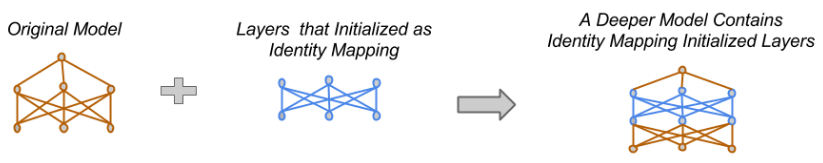
\includegraphics[scale=0.3]{images/net2deepernet.png}
        \end{centering}
    \end{figure}

}

%----------------------------------------------------
\begin{frame}{Network Morphisms Allow Efficient Moves in Architecture Space }

    \begin{figure}[t]
        \begin{centering}
%            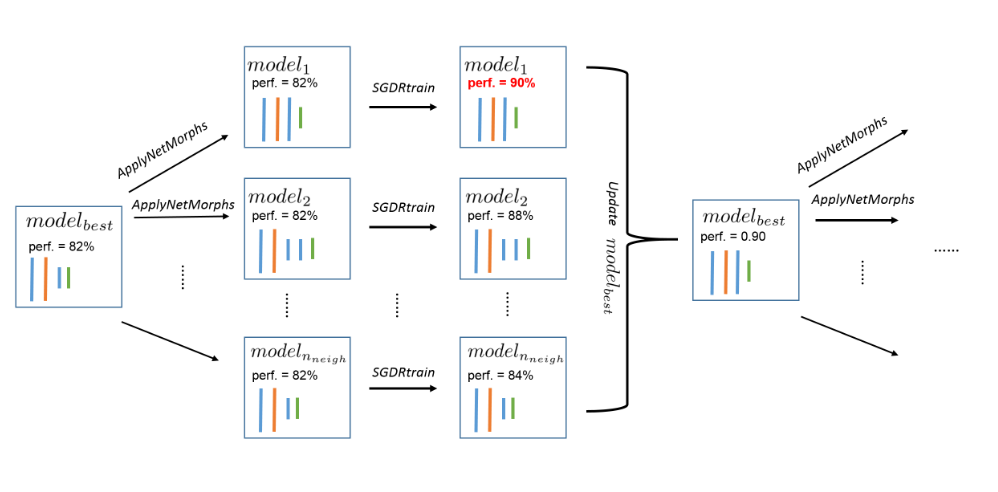
\includegraphics[scale=0.3]{images/NASH.png}
            \onslide<1->{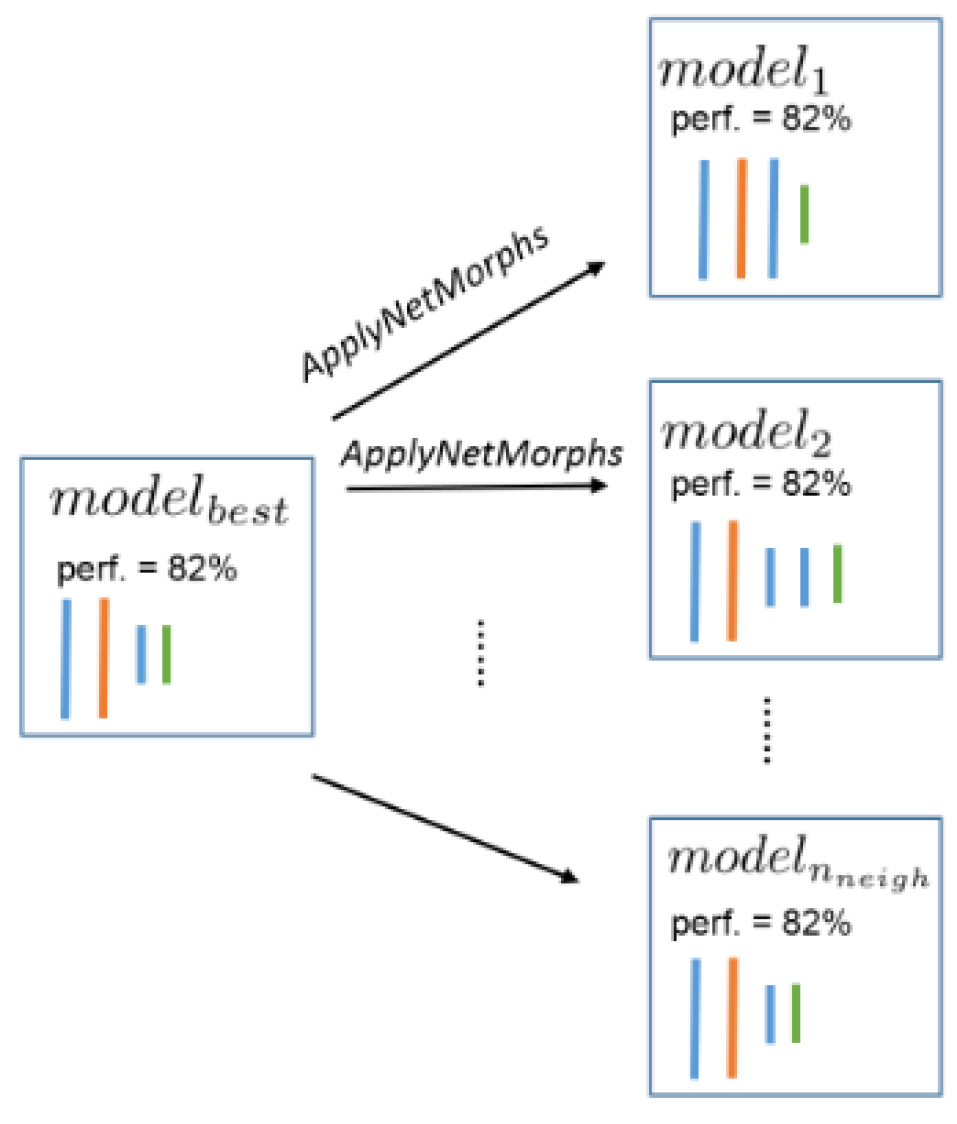
\includegraphics[scale=0.36]{images/NAS_with_greedy_morphisms_1.png}}
            \onslide<2->{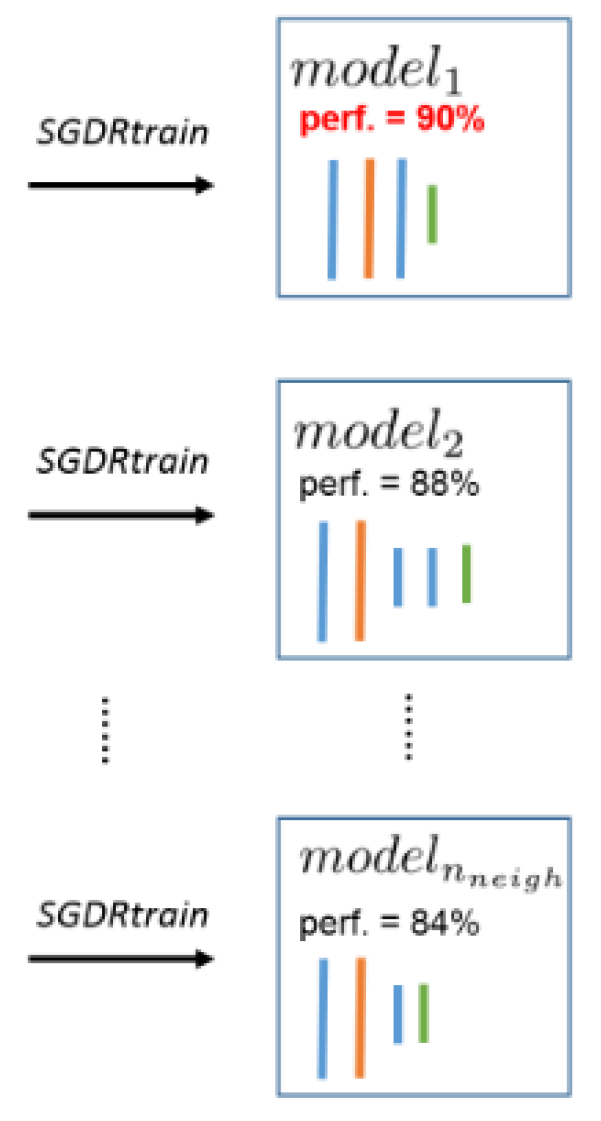
\includegraphics[scale=0.36]{images/NAS_with_greedy_morphisms_2.png}}
%			\onslide<3->{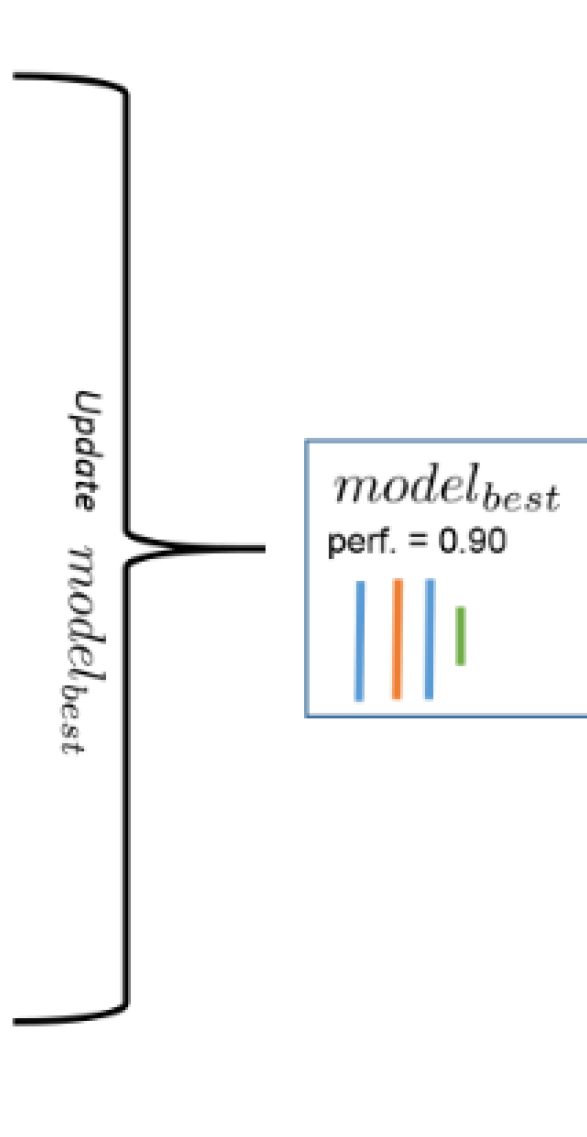
\includegraphics[scale=0.36]{images/NAS_with_greedy_morphisms_3.png}}
            \onslide<3->{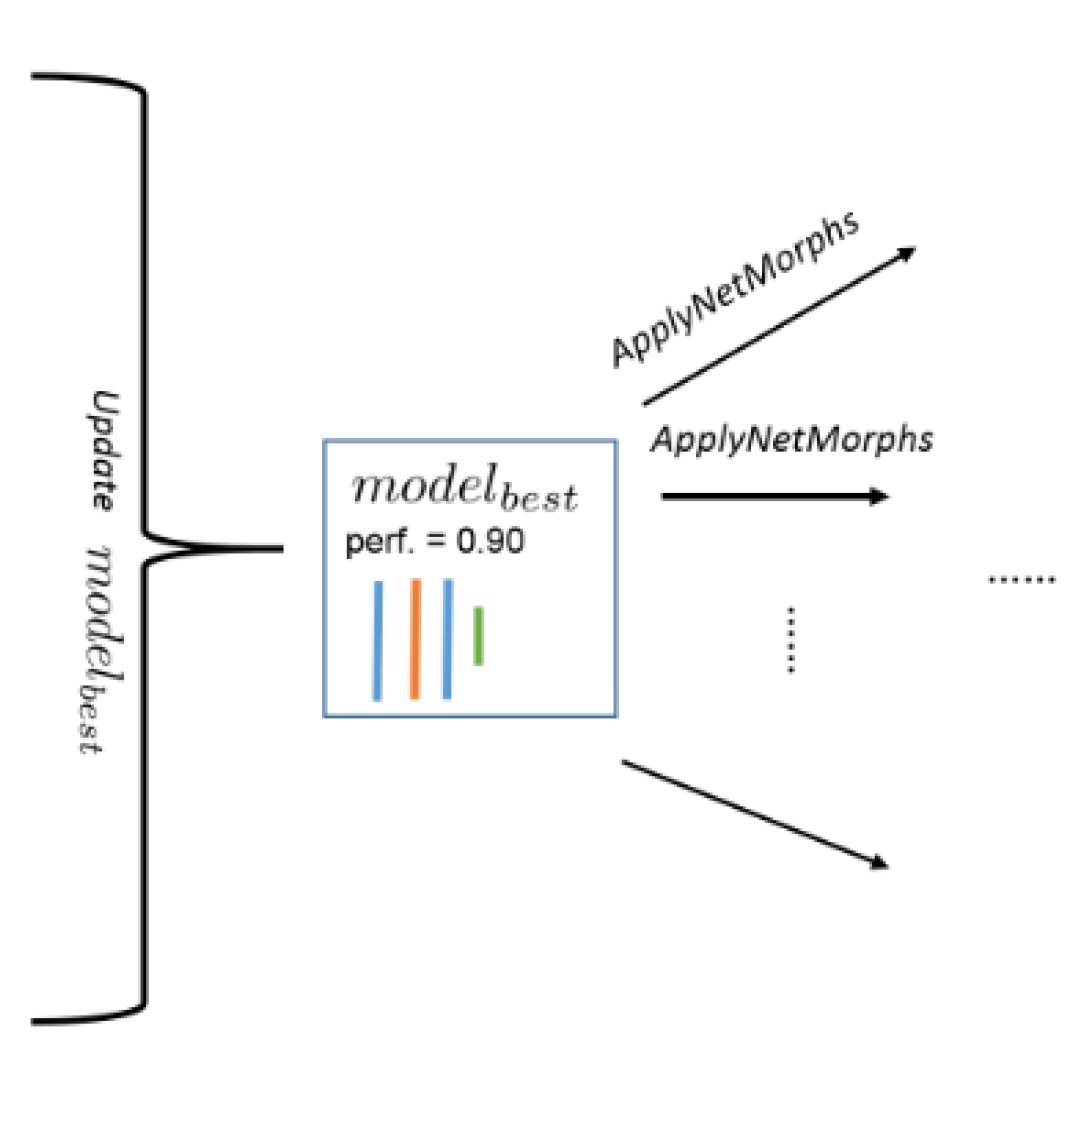
\includegraphics[scale=0.36]{images/NAS_with_greedy_morphisms_4.png}}	
         \end{centering}
    \end{figure}

\begin{center}
\onslide<4->{
	\alert{Weight inheritance} avoids expensive retraining from scratch\\
	\lit{\href{https://arxiv.org/pdf/1703.01041.pdf}{Real et al. 2017}; \href{https://www.aaai.org/ocs/index.php/AAAI/AAAI18/paper/viewFile/16755/16568}{Cai et al. 2018}; \href{http://metalearning.ml/2017/papers/metalearn17_elsken.pdf}{Elsken et al. 2017}; \href{http://proceedings.mlr.press/v70/cortes17a/cortes17a.pdf}{Cortes et al. 2017}; \href{http://proceedings.mlr.press/v80/cai18a/cai18a.pdf}{Cai et al. 2018}; \href{https://openreview.net/pdf?id=ByME42AqK7}{Elsken et al. 2019}}
}
\end{center}

\end{frame}
%----------------------------------------------------

%----------------------------------------------------
\myframetop{Network Morphisms for Multi-objective NAS \litw{\href{https://openreview.net/pdf?id=ByME42AqK7}{Elsken et al. 2019}}}{

	\myit{
		\item To trade off error vs. resource consumption (e.g, \#parameters): 
		\myit{
			\item Maintain a \alert{Pareto front} of the two objectives
			\item Evolve a population of Pareto-optimal architectures over time
		}			
	}
    \begin{center}
    \only<1>{
    	\vspace*{0.35cm}
    	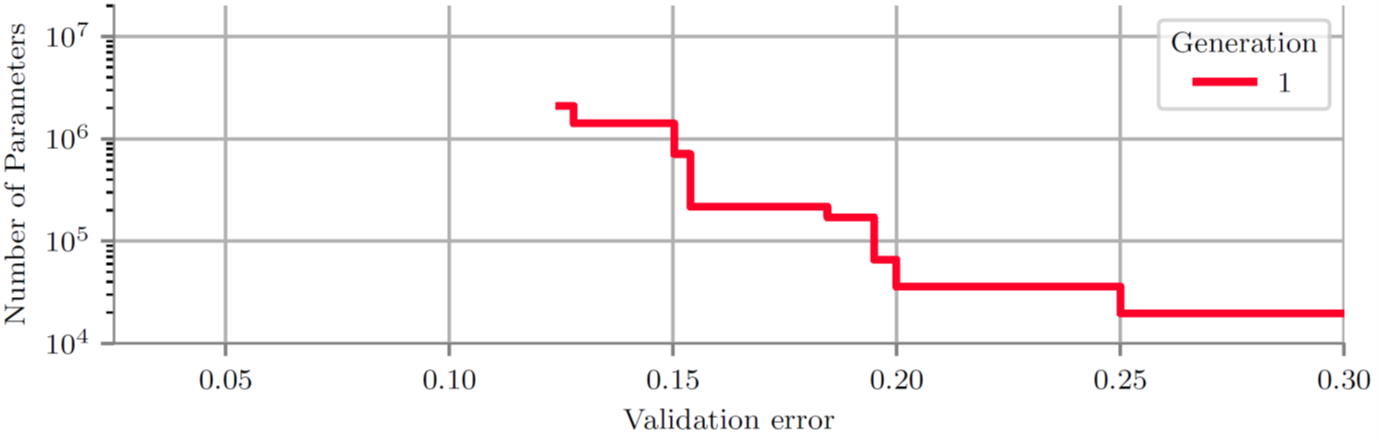
\includegraphics[width=0.78\textwidth]{images/lemonade_generation1.png}
    }
    \only<2>{
    \hspace*{-0.15cm}
    	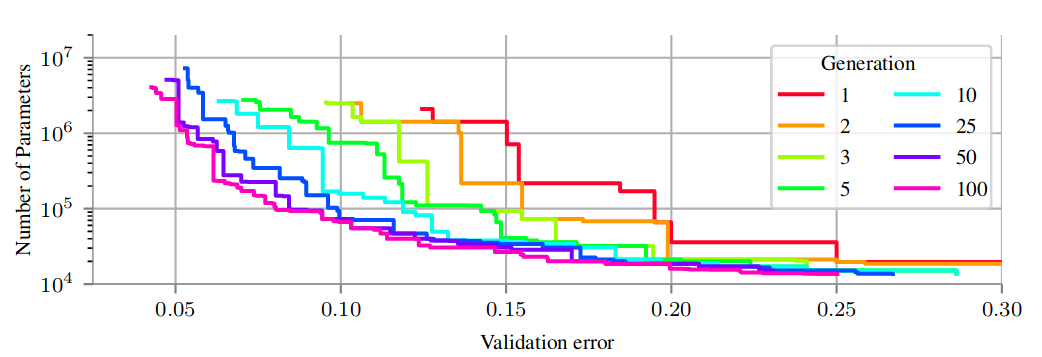
\includegraphics[width=0.8\textwidth]{images/lemonade.png}
	}
    \end{center}
}
%----------------------------------------------------



%----------------------------------------------------
\myframe{Network Morphisms for Multi-objective NAS \litw{\href{https://openreview.net/pdf?id=ByME42AqK7}{Elsken et al. 2019}}}{
	\myit{
		\item \alert{LEMONADE}: \alert{L}amarckian \alert{E}volution for \alert{M}ulti-\alert{O}bjective \alert{N}eural \alert{A}rchitecture \alert{De}sign
  		\item Weight inheritance through approximate morphisms (ANMs)
		\myit{
			\item Dropping layers, dropping units within a layer, etc (function not preserved perfectly)
%			\item Still cheap: e.g., 1 week on 8 GPUs
		}
	}
    \begin{figure}[t]
        \begin{center}
    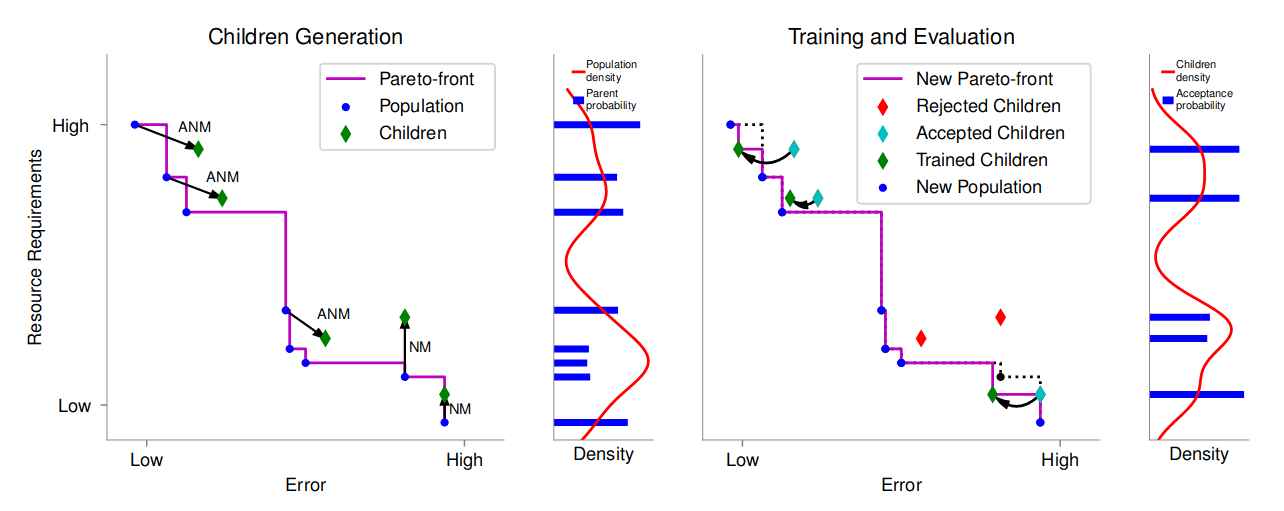
\includegraphics[scale=0.30]{images/lemonade_2.png}
        \end{center}
    \end{figure}
}
%----------------------------------------------------


%----------------------------------------------------------------------
\myframetop{NAS Speedup Technique 5: Weight Sharing and One-shot Models \\ \litw{\href{https://arxiv.org/pdf/1802.03268.pdf}{Pham et al. 2018}; \href{http://proceedings.mlr.press/v80/bender18a/bender18a.pdf}{Bender et al. 2018}}}{
\centering
	\myit{
		\item All possible architectures are subgraphs of a large supergraph: 
		the \alert{one-shot model}
\medskip
\pause
		\item \alert{Weights are shared} between different architectures with common edges in the supergraph
\medskip
\pause
		\item \alert{Search costs are reduced} drastically since one only has to train a single model (the one-shot model).\\
	}

%	\centering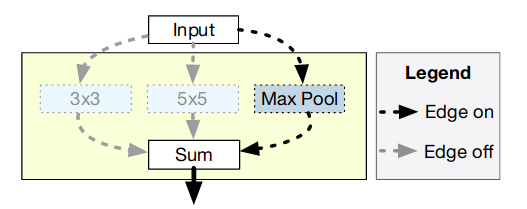
\includegraphics[width=0.5\textwidth]{images/one_shot_nas.png}
%	\pause
%	\item Different one-shot NAS methods differ in how the train the one-shot model and sample
%	from it:
%	\begin{itemize}
%            \item[$\Rightarrow$] ENAS \lit{Pham et al, 2018} uses an RL controller to sample architectures from the supergraph and trains the one-shot model using on approximate gradients obtained through REINFORCE
%            \item[$\Rightarrow$] Bender et al. (18) only train the one-shot model and sample architectures in the end
%	    \item[$\Rightarrow$] DARTS (Differentiable Architecture Search; \lit{Liu et al, 2018}) creates a continuous relaxation of the discrete architecture space and optimizes the architecture distribution with gradient descent
%	\end{itemize}
%	\end{itemize}
	
}


%----------------------------------------------------
\myframetop{NAS Speedup Technique 5: Weight Sharing and One-shot Models\\ \litw{\href{https://arxiv.org/pdf/1802.03268.pdf}{Pham et al. 2018}; \href{http://proceedings.mlr.press/v80/bender18a/bender18a.pdf}{Bender et al. 2018}}}{

	\myit{
		\item The one-shot model can be seen as a \alert{directed acyclic multigraph}
		\begin{itemize}
	            \item[$\Rightarrow$] \alert{Nodes} - latent representations.
	            \item[$\Rightarrow$] \alert{Edges} (dashed) - operations.
	        \end{itemize}
    }
	
	\begin{centering}
    	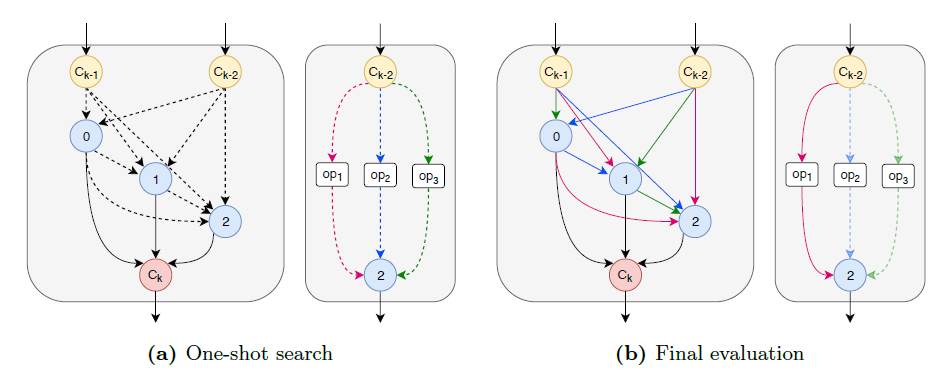
\includegraphics[scale=0.47]{images/cell_space.png}
	\end{centering}
	
	\myit{
		\item Architecture optimization problem: \alert{Find optimal path from the input to the output}
	}
	
}
%----------------------------------------------------



%----------------------------------------------------------------------
\myframe{Questions to Answer for Yourself / Discuss with Friends}{

	\myit{
		\item Repetition:\\\alert{List five methods to speed up NAS over blackbox approaches}
		\medskip
		\item Repetition:\\\alert{Which speedup techniques directly carry over from HPO to NAS?}
		\medskip
		\item Discussion:\\\alert{Why do network morphisms and the one-shot model only apply to NAS, and not to HPO?}
%		\medskip
%		\item Transfer:\\\alert{Discuss the similarities between the one-shot model and dropout training}
	}
}
%-----------------------------------------------------------------------
